
	\chapter{Analisi cinematica dei meccanismi con coppie a camma}
	
		\section{Introduzione}
		
		\begin{minipage}{.7\textwidth}
		L'analisi cinematica dei meccanismi a camma ha lo scopo di determinare la relazione tra le grandezze cinematiche del cedente e del movente, note la geometria e la forma dei profili coniugati.
		
		Il movente è collegato al telaio generalmente da una coppia rotoidale; la camma che funge da cedente può essere invece collegata al telaio sia da una coppia rotoidale che prismatica. Si ha nel primo caso un cedente oscillante (\emph{bilanciere}) e nel secondo caso un cedente dotato di moto traslatorio (\emph{punteria}). Nella figura è rappresentata una tipica applicazione a camma.
		
		Alcuni meccanismi con coppie a camma sono immediatamente riconducibili a meccanismi con sole coppie elementari (\emph{prismatiche e rotoidali}).
		
		Consideriamo il meccanismo a glifo oscillante formato da tre membri rigidi (\emph{uno telaio}) connessi tramite due coppie rotoidali ed una coppia a camma. Esso possiede un grado di libertà, infatti applicando la formula di Grübler otteniamo:
		\[n = 3(m-1) - 2c_1 - 1c_2 = 3(3-1)-2\cdot2 -1\cdot1 = 1\]
		
		\end{minipage}
		\hfill
		\begin{minipage}{.25\textwidth}
		\centering
		\includegraphics[width=0.9\textwidth]{chapter04/Immagine74}	
		\end{minipage}
		\vspace{2mm}
		
		Questo meccanismo è completamente analogo dal punto di vista cinematico al meccanismo a glifo oscillante con sole coppie elementari. I 2 G.d.L rappresentati dal moto relativo tra i due membri 1 e 2 e lasciati liberi \textbf{dalla coppia a camma sono associati alla traslazione del pattino ed alla rotazione della coppia rotoidale}.
		
		\begin{figure}[!h]
		\centering
		\includegraphics[width=0.8\textwidth]{chapter04/Immagine75}
		\end{figure}
 
		Quello che distingue i due meccanismi è la meccanica del contatto, nel meccanismo con coppia a camma vi è un contatto di tipo lineare, mentre nel meccanismo con sole coppie elementari vi è un contatto tra superfici estese.
		
		** Svolgento il calcolo dei G.d.L. tramite la formula di Grübler del meccanismo equivalente deve essere tenuta in considerazione l'introduzione di un corpo aggiuntivo, ovvero il pattino.
		
		Nel seguito mostreremo come anche altri meccanismi con coppie a camma siano riconducibili, anche se in maniera meno immediata, a dei meccanismi con sole coppie elementari. 
		
		Intraprendiamo ora lo studio cinematico dei meccanismi che sono comunemente chiamati meccanismi a camma (\emph{anche se non sono i soli a contenere la coppia a camma}). Essi sono costituiti da un telaio, un membro rigido chiamato camma, collegato al telaio tramite una coppia rotoidale o prismatica, un secondo membro rigido, chiamato cedente, collegato al telaio pure da una coppie rotoidale o prismatica.
		
		Il \textbf{membro motore è la camma}, la parte della sua superficie che entra in contatto con il cedente viene chiamata profilo della camma ed è realizzata in modo tale da impartire un particolare movimento desiderato al cedente; si realizza così un meccanismo nel quale la posizione del cedente è una \textbf{opportuna funzione della posizione della camma}. Il cedente è mantenuto in contatto con la camma con accoppiamento di forma o di forza.
		
		I meccanismi a camma spesso sono la soluzione più semplice per realizzare dei moti complessi con alta ripetibilità ed affidabilità, perciò sono molto diffusi nelle applicazioni industriali. 
		
		A titolo di esempio le camme a disco sono le più usate e sono diffusamente impiegate nei motori a combustione interna, nei timer, e nelle macchine utensili; gli altri tipi di camme sono meno diffusi e trovano impiego soprattutto nelle macchine automatiche. Per questa ragione accentreremo il nostro interesse sulle camme a disco.\newline
			
		Consideriamo dunque il meccanismo proposto nella figura a lato:
				\vspace{2mm}
		
		\begin{minipage}{.3\textwidth}
		\centering
		\includegraphics[width=.95\textwidth]{chapter04/Immagine76}
		\end{minipage}
		\hfill
		\begin{minipage}{.7\textwidth}
	
		
		Scelta come coordinata generalizzata la rotazione \emph{q} del sistema solidale alla camma rispetto al sistema fisso, lo spostamento lineare (\emph{cedente traslante}) o angolare (\emph{cedente oscillante}) del cedente viene espresso in funzione della rotazione della camma tramite la funzione di spostamento $s = f(q)$, il suo diagramma è chiamato diagramma delle alzate
		

		\centering
		\includegraphics[width=.5\textwidth]{chapter04/Immagine78}
		\end{minipage}
		
		Un tipico diagramma delle alzate è il seguente (\emph{lo spostamento del cedente può essere lineare o angolare}), esso è suddiviso in quattro fasi:
		\begin{enumerate}[$\Rightarrow$]
		\item \textbf{fase di salita}, nella quale la rotazione della camma passa da $q_0$ a $q_1$ e nella quale corrispondentemente lo spostamento del cedente passa da 0 al valore massimo;
		\item \textbf{fase di sosta}, nella quale la rotazione della camma passa da $q_1$ a $q_2$ e corrispondentemente lo spostamento del cedente si mantiene al valore massimo;
		\item \textbf{fase di ritorno}, nella quale la rotazione della camma passa da $q_2$ a $q_3$ e corrispondentemente lo spostamento del cedente passa dal valore massimo a zero;
		\item \textbf{fase di sosta}, nella quale la rotazione della camma passa da $q_3$ a $q_0 + 2 \pi$ (\emph{completamento del ciclo}) e corrispondentemente il cedente non si sposta
		\end{enumerate} 
		
		\begin{minipage}{.5\textwidth}
		\centering
		\includegraphics[width=.8\textwidth]{chapter04/Immagine77}
		\end{minipage}
		\hfill
		\begin{minipage}{.5\textwidth}
		La posizione H(q) = f(s) del cedente è legata alla funzione di spostamento, nei casi più semplici dalla formula:
		\[
		H(q) = s(q) + H(q_0)
		\]
		
		Tramite l'introduzione di tale relazione possiamo svolgere l'analisi cinematica del meccanismo:
		
			\begin{gather*}
		\dot{H} = \td{H}{t} = \td{s}{q}\,\td{q}{t} = s'(q)\,\dot{q} \\
		 *\text{s(q): s dipende dal profilo geometrico della camma}\\
		\tau_{H,q} = \frac{\dot{H}}{\dot{q}} = s'(q)\\
		\end{gather*}
		\end{minipage}
		
	s'(q) è dunque il rapporto di velocità tra cedente e movente. Proseguiamo con l'analisi di accelerazione

	
		
		\begin{align*}
		\ddot{H} = \td{(s'(q)\,\dot{q})}{t}&= s'(q)\,\dot{q} + (\td{s'(q)}{t})\,\dot{q}\\
		&= s'(q) \,\ddot{q} + \td{s'(q)}{q}\,\td{q}{t}\,\dot{q}\\
		&= s'(q) \,\ddot{q} + \td{s'(q)}{q}\,\dot{q}^2\\
		&= s'(q) \,\ddot{q} + s''(q)\,\dot{q}^2
		\end{align*}
		
		Possiamo notare che anche l'accelerazione del cedente è proporzionale all'accelerazione del movente tramite il fattore s'(q), che ricordiamo ancora una volta, è un contributo geometrico.\newline
		
		Un secondo fattore di proporzionalità è dato tra l'accelerazione del movente e la velocità del cedente al quadrato (s''(q)): tale fattore suggerisce che anche se l'angolo q sta girando con velocità angolare costante, dà ugualmente un contributo all'accelerazione del cedente.
		
		Devo preoccuparmi, dunque, che tale termine sia sufficientemente regolare (ha un significato dinamico importante): un profilo di velocità (s'(q)) con presenza di discontinuità produrrà un profilo di accelerazione altrettanto pieno di discontinuità indesiderate (si faccia riferimento al terzo principio della dinamica).
		
		Per avere un movimento regolare del cedente la derivata prima della funzione di spostamento rispetto a q deve essere continua anche nei punti di transizione e possibilmente anche la derivata seconda deve essere continua nei punti di transizione.
		
		Discontinuità di s'(q) provocano discontinuità della velocità del cedente e quindi accelerazioni teoricamente infinite e forze d'inerzia inammissibilmente elevate. Discontinuità di s''(q) provocano discontinuità dell'accelerazione del cedente e quindi discontinuità della forza di contatto tra camma e cedente, che producono vibrazioni ed usura accelerata.
		
		Poiché abbiamo visto che la posizione del cedente è legata alla funzione di spostamento, la velocità del cedente è legata alla derivata rispetto a q della funzione di spostamento, l'accelerazione del cedente è legata alle derivate prima e seconda della funzione di spostamento, il problema di analisi cinematica dei meccanismi a camma può essere riformulato nel seguente modo: \textbf{data una camma già realizzata determinare la funzione di spostamento del cedente e le sue derivate}.
		
		\section{Analisi cinematica dei meccanismi a camma con il metodo dell'equivalenza cinematica}
		
		Come primo esempio consideriamo una camma a cerchio eccentrico completo e cedente traslante a rotella (\emph{punteria a rotella}).
		

		\begin{center}
		\includegraphics[width=.6\textwidth]{chapter04/Immagine80}
		\end{center}
		
		Scegliamo il sistema solidale all'asse $x_m$ passante per il centro del cerchio. In questo caso durante il movimento, grazie alla geometria del profilo ad arco di cerchio e della rotella, la distanza tra centro del cerchio e centro della rotella rimane costante e pari alla somma dei raggi del cerchio R e della rotella r, poiché le normali devono rimanere allineate e coincidenti con i raggi.
		
		Anche la distanza tra il centro dell'arco di cerchio e il centro di rotazione della camma è costante e pari all'eccentricità ``e'' della camma.
		
		Il meccanismo a camma perciò si muove come un equivalente meccanismo di spinta avente la manovella lunga e, la biella 2 lunga (R+r) e il pattino 3 coincidente con il cedente traslante.
		
		Per ricavare la funzione di spostamento si effettua l'analisi di posizione del meccanismo articolato equivalente. Si traccia il poligono di chiusura; scelto il verso di percorrenza possiamo scrivere l'equazione:
		
				\begin{gather*}
				\mathbf{AB} +\mathbf{BC} + \mathbf{CD} + \mathbf{DA}=0\\
				l\,\B{\cos{q}\\\sin{q}}\,+\,(R+r)\,\B{\cos{\theta_2}\\\sin{\theta_2}} + s\,\B{0\\-1}\,+d\,\B{-1\\0}=0\\
				\begin{cases}
				(R+r)\,\cos{\theta_2} = d-e\cos{q}\\
				(R+r)\,\sin{\theta_2} = s - e \sin{q}
				\end{cases}\\
				\text{elevando le equazioni sopra definite e sommandole membro a membro si ottiene}\\
				(R+r)^2	 = d^2 + e^2 + s^2 -2e\,d\cos{q} -2e\,s\sin{q}\\
				\text{risolvendo tale equazione di secondo grado si possono ottenere due soluzioni della funzione di spostamento:}\\
				s_{1,2} = e\sin{q} \pm \sqrt{(R+r)^2 - d^2 - e^2\cos{q}^2 + 2e\,d\cos{q}}\\
				\text{Noto che non è di utilità un valore negativo di s(q), possiamo concludere che la soluzione di nostro interesse è:}\\
				s = e\sin{q} + \sqrt{(R+r)^2 - d^2 - e^2\cos{q}^2 + 2e\,d\cos{q}}\\
				\end{gather*}
		
		Proseguiamo l'analisi cinematica del meccanismo con l'analisi di velocità:
		
		\begin{align*}
		\M{-(R+r)\sin{\theta_2}&0\\(R+r)\cos{\theta_2}&-1}\,\B{\dot{\theta_2}\\\dot{s}} &= \B{e\sin{q}\\-e\cos{q}}\,\dot{q}\\
		\B{\dot{\theta_2}\\\dot{s}} &= \frac{1}{(R+r)\sin{\theta_2}}\,\M{-1&0\\-(R+r)\cos{\theta_2}&-(R+r)\sin{\theta_2}}\,\B{e\sin{q}\\-e\cos{q}}\,\dot{q}
		\end{align*}
		
		Da cui possiamo ricavare il rapporto di velocità tra cedente s e movente e successivamente l'espressione di s'(q):
		\begin{gather*}
		\dot{s} = \underbrace{e\,\frac{\sin{(\theta_2 - q)}}{\sin{\theta_2}}}_{\tau_{s,q}}\,\dot{q}\\
		\td{s}{q} = s' = \td{s}{q} \td{t}{q} = \tau_{s,q} = e\,\frac{\sin{(\theta_2 - q)}}{\sin{\theta_2}}
		\end{gather*}
		
		Per concludere svolgiamo l'analisi d'accelerazione:
		\begin{equation*}
		\tdd{s}{q} = s'' = \td{\tau_{s,q}}{q} =  \frac{e\,\sin{(\theta_2 - q)}\,\td{(\theta_2-q)}{q}\,\sin{\theta_2}\,-\,\sin{\theta_2-q}\,\cos{\theta_2}\,\td{\theta_2}{q}}{\sin{\theta_2}^2}
		\end{equation*}
		
		\section{Analisi cinematica dei meccanismi con l'equazione ausiliaria}
		
		Per descrivere il profilo di una camma di forma arbitraria rispetto al sistema di riferimento solidale avente origine nella coppia rotoidale fissa si introducono le coordinate polari $\rho$ e $\beta$, dove $\rho$ è il modulo del raggio che unisce l'origine del sistema solidale al generico punto P del profilo e $\beta$ è l'angolo (\emph{positivo se antioriario}) compreso tra l'asse $x_m$ e il raggio stesso.
		
		Facendo uso di questa notazione il profilo è espresso matematicamente da una funzione $\rho(\beta)$.
		
		\begin{minipage}{.65\textwidth}
		Per effettuare l'analisi cinematica si deve conoscere anche l'angolo $\nu$ formato dal raggio con la normale n al profilo nel punto P di contatto con il cedente.
		
		Se la tangente t è orientata secondo il verso positivo di rotazione intorno a $z_m$ e la normale n è orientata in modo tale da sovrapporsi alla tangente con una rotazione di $+\pi/2$, allora $\nu$ può essere espresso in funzione di $\beta$ nella forma:
		\[
		\nu = \nu(\beta) = \arctan{\frac{-\td{\rho}{\beta}}{\rho}}
		\]
		
		Stabilite queste definizioni intraprendiamo l'analisi di alcuni meccanismi a camma:
		\end{minipage}
		\hfill
		\begin{minipage}{.35\textwidth}
		\centering
		\includegraphics[width = .85\textwidth]{chapter04/Immagine81}
		\end{minipage}
		
		\subsection{Camma a disco con punteria a piattello}
		
		Per prima cosa si stabiliscono i S.d.R. fisso e solidale entrambi con origine nel centro della coppia rotoidale fissa; la coordinata generalizzata q è la rotazione tra sistema fisso e sistema solidale.
		
		La posizione del punto di contatto P varia nel tempo sia rispetto al S.d.R. fisso che rispetto al sistema di riferimento mobile ed è definita dal vettore $\mathbf{AP}$ che è inclinato idi $\beta$ (variabile) rispetto al sistema solidale e di ($\beta + q$) rispetto al sistema fisso; il modulo di $\mathbf{AP}$ è proprio il raggio $\rho$ della camma, che come è noto è funzione di $\beta$.
		
		Chiamiamo M il punto al centro del piattello. Stabilito il verso di percorrenza si può srivere l'equazione di chiusura in forma vettoriale e scalare:
		
		\begin{gather*}
		\mathbf{AP} + \mathbf{PM} + \mathbf{MB} + \mathbf{BA} = 0\\
		\rho(\beta)\,\B{\cos{(q+\beta)}\\\sin{(q+\beta)}} + a\,\B{1\\0} + s\B{0\\-1} + d\B{-1\\0} = 0
		\end{gather*}
		
		q è noto in quanto coordinata generalizzata, le incognite del problema, di conseguenza, risultano essere: $\beta, a ,s$ (2 equazioni in 3 incognite).
		
		Questo sistema di due equazioni non lineari contiene 3 incognite e non è sufficiente a risolvere il problema cinematico, ciò deriva dal fatto che il punto di contatto tra camma e cedente non è noto.
		
		Si può aggiungere una terza equazione scrivendo la condizione che esprime la concidenza della normale alla camma con la normale al piattello nel punto di contatto P; infatti la camma e piattello sono due profili coniugati e devono avere normali e tangenti coincidenti nel punto di contatto. Poiché la normale al piattello è inclinata di $\pi/2$ rispetto all'orizzontale, dalla figura si ottiene:
		
		\[q+\beta +\nu(\beta) = \pi/2\]
		
		\section{Camma con cedente oscillante a rotella}
		
		
\begin{minipage}{.5\textwidth}
		Come secondo esempio consideriamo l'analisi cinematica di un meccanismo a camma con profilo generico e cedente oscillante a rotella.
		
		Si stabiliscono un sistema di riferimento fisso ed uno mobile solodale alla camma, entrambi con origine nella rima coppia rotoidale fissa, la coordinata generalizzata q è proprio la rotazione da sistema fisso a sistema mobile.
		
		La posizione del punto di contatto P è definita dal vettore $\mathbf{AB}$, che è inclinato di $\beta$ rispetto al sistema mobile e di $\beta + q$ rispetto al sistema fisso ed ha modulo $\rho(\beta)$.
		
		Chiamiamo $\und{PB}$ il vettore (\emph{allineato con il raggio della rotella}), che unisce il punto di contatto P al centro della rotella. 
		\end{minipage}
		\hfill
		\begin{minipage}{.5\textwidth}
		\centering
		\includegraphics[width=.8\textwidth]{chapter04/Immagine83}
		\end{minipage}
		\vspace{2mm}
		
		Chiamiamo $\mathbf{BC}$ il vettore che unisce la seconda coppia rotoidale fissa al centro della rotella. Infine chiamiamo $\mathbf{AC}$ il vettore che unisce le due coppie rotoidali fisse.
		 Possiamo tracciare il seguente poligono di chiusura.
		\vspace{2mm}
		
		\begin{minipage}{0.5\textwidth}
		\centering
		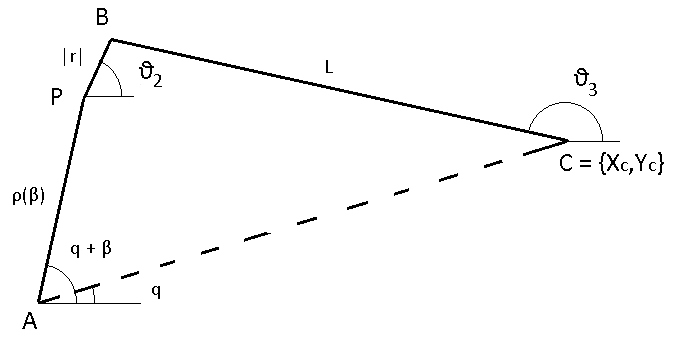
\includegraphics[width=0.9\textwidth]{chapter04/Immagine84}
		\end{minipage}
		\hfill
		\begin{minipage}{0.5\textwidth}
		
		 Stabilito il verso di percorrenza si può scrivere l'equazione vettoriale di chiusura:
		
		\[\mathbf{AP}+\mathbf{PB}+\mathbf{BC}+\mathbf{CA} = 0\]
		
		che in termini scalari fornisce:
		
		\[
		\rho(\beta)\,\B{\cos{(q +\beta)}\\\sin{(q+\beta)}} + r\,\B{\cos{\theta_2}\\\sin{\theta_2}} + L\,\B{-\cos{\theta_3}\\-\sin{\theta_3}} + \B{-x_C\\-y_C}
		\]
		\end{minipage}
		\vspace{2mm}
		
		Noto il movente ``q'' le variabili incognite risultano essere $\theta_2$, $\theta_3$ e $\beta$. Tuttavia il poligono di chiusura tracciato propone solamente 2 equazioni in 3 incognite: sarà dunque necessario utilizzare l'equazione ausiliaria.
		\[
		q + \beta(q) + \nu(\beta) = \theta_2
		\]

	